%%%%%%%%%%%%%%%%%%%%%%%%%%%%%%%%%%%%%%%%%
% Stylish Article
% LaTeX Template
% Version 2.2 (2020-10-22)
%
% This template has been downloaded from:
% http://www.LaTeXTemplates.com
%
% Original author:
% Mathias Legrand (legrand.mathias@gmail.com) 
% With extensive modifications by:
% Vel (vel@latextemplates.com)
%
% License:
% CC BY-NC-SA 3.0 (http://creativecommons.org/licenses/by-nc-sa/3.0/)
%
%%%%%%%%%%%%%%%%%%%%%%%%%%%%%%%%%%%%%%%%%

%----------------------------------------------------------------------------------------
%	PACKAGES AND OTHER DOCUMENT CONFIGURATIONS
%----------------------------------------------------------------------------------------

\documentclass[fleqn,10pt]{SelfArx} % Document font size and equations flushed left

\usepackage[english]{babel} % Specify a different language here - english by default

\usepackage{lipsum} % Required to insert dummy text. To be removed otherwise

%----------------------------------------------------------------------------------------
%	COLUMNS
%----------------------------------------------------------------------------------------

\setlength{\columnsep}{0.55cm} % Distance between the two columns of text
\setlength{\fboxrule}{0.75pt} % Width of the border around the abstract

%----------------------------------------------------------------------------------------
%	COLORS
%----------------------------------------------------------------------------------------

\definecolor{color1}{RGB}{0,0,90} % Color of the article title and sections
\definecolor{color2}{RGB}{0,20,20} % Color of the boxes behind the abstract and headings

%----------------------------------------------------------------------------------------
%	HYPERLINKS
%----------------------------------------------------------------------------------------

\usepackage{hyperref} % Required for hyperlinks

\hypersetup{
	hidelinks,
	colorlinks,
	breaklinks=true,
	urlcolor=color2,
	citecolor=color1,
	linkcolor=color1,
	bookmarksopen=false,
	pdftitle={Title},
	pdfauthor={Author},
}

%----------------------------------------------------------------------------------------
%	ARTICLE INFORMATION
%----------------------------------------------------------------------------------------

\JournalInfo{Assignment 1 - Machine Learning for Natural Language Processing} % Journal information
\Archive{Fall Semester 2022} % Additional notes (e.g. copyright, DOI, review/research article)

\PaperTitle{Can twitter predict language? A computational approach to language classification} % Article title

\Authors{Kiram Ben Aleya\textsuperscript{1}*, Kilian Sennrich\textsuperscript{2}*} % Authors
\affiliation{\textsuperscript{1}\textit{Department of Computer Science, University of Zurich, Altstetten, Switzerland}} % Author affiliation
\affiliation{\textsuperscript{2}\textit{Department of Computer Science, University of Zurich, Unterentfelden, Switzerland}} % Author affiliation
\affiliation{*\textbf{Corresponding authors}: kiram.benaleya@uzh.ch, killian.sennric@uzh.ch} % Corresponding author

\Keywords{NLP --- Language Classification --- Linear Classifier --- Deep Neural Nets} % Keywords - if you don't want any simply remove all the text between the curly brackets
\newcommand{\keywordname}{Keywords} % Defines the keywords heading name

%----------------------------------------------------------------------------------------
%	ABSTRACT
%----------------------------------------------------------------------------------------

\Abstract{Classifying Language is an essential component of almost every Natural Language Processing (NLP) pipeline. Working with mulitilingual data often requires Machine Translation (MT) as a preprocessing step. Some Libraries for MT in Python and R do not provide automatic language detection, which poses an issue if, exampli gratia, one works with a corpus containing documents in dozens of different languages, as appears in scraped twitter data. In this paper, we describe our findings of a machine learning approach to automatically detect languages. In particular we trained our models directly on twitter data, which might be an advantage over existing models when working with this type of data. This paper is not meant to be an academic paper, but rather an informal description of our project. We will outline our preprocessing, and detail our models. In particular we trained a Logistic Regression Model, which serves as a baseline. We compare this to our second model, which is of deep neural nature. We find that the Logistic Regression Model outperformed the Neural Net by about 50\%. These results are not expected to be robust as we had to optimize for computational workload. }

%----------------------------------------------------------------------------------------

\begin{document}

\maketitle % Output the title and abstract box

\tableofcontents % Output the contents section

\thispagestyle{empty} % Removes page numbering from the first page

%----------------------------------------------------------------------------------------
%	ARTICLE CONTENTS
%----------------------------------------------------------------------------------------

\section{Introduction} % The \section*{} command stops section numbering

This is the our report for the first assignment of the Machine Learning for Natural Language Processing 1 course. The task was to train a linear, as well as a Deep Neural Net model on twitter data, which can predict the language of the tweet. The goal of this exercise is to: 

\begin{itemize}[noitemsep] % [noitemsep] removes whitespace between the items for a compact look
	\item understand linear models and use them for multiclass classification tasks
	\item be able to implement different machine learning models, including MLPs, in scikit-learn
	\item understand the role of hyper-parameters, regularisation, and the problems of class imbalance.
	\item perform an error analysis of machine learning models.
	\item observe the most important features that lead to a prediction of a specific class and explains to some degree what the model does (XAI).
\end{itemize}

\section{Task \& Data Description}

\subsection{Data}

For both parts of this exercise, we will work with the same data. The goal is to classify the language of twitter tweets. This is a challenging extension of the problem described in Goldberg, chapter 2. However, we will work with more languages than just six and the text segments we need to classify are much shorter. The material folder in the exercise section on OLAT contains the two files “train\_dev\_set.tsv” and “test\_set.tsv”. 

\subsection{Tasks}

\paragraph{Task 1} Scikit-learn is a useful Python library for all kinds of machine learning tasks. In the following, you will train several models in sklearn to solve this task. The aim is to become acquainted with a few different classifiers, as well as with the basic functionality of sklearn.
\begin{enumerate}[noitemsep] % [noitemsep] removes whitespace between the items for a compact look
	\item Create a suitable pipeline in sklearn to preprocess the data. Think about extending the feature space. What other features could you use to determine the language? Please include extra features linguistic features to your machine learning model for this task.
	\item  Train the following classifier: LogisticRegression
	\item To find the optimal hyperparameter settings for the classifier, use sklearn’s GridSearchCV. You are supposed to experiment with the following hyperparameters: Penalty (Regularisation), Solver,  Experiment with parameters of the Vectoriser (not required, highly advised).
\end{enumerate}

Report the hyperparameter combination for your best-performing model on the test set. What is the advantage of grid search cross-validation? Use a confusion matrix to do your error analysis and summarize your answers in your report. Now that you have your best model, it’s time to dive deep into understanding how the model makes predictions. It is important that we can explain and visualize our models to improve task performance. 

Explainable models help characterize model fairness, transparency, and outcomes. Let's try to understand what our best performing logistic regression classification model has learned. Generate a feature importance table for the top ten features (please have the features named) for the languages [‘en, ‘es’, ‘ja’]. What is more important, extra features or the outputs of the vectorizer, discuss. We recommend using the ELI5 library as it supports sklearn pipelines to explain the model weights. For more details, see their documentation on dealing with text classification. We will accept answers from any explanation library/method as long as the explanations for the model weights are provided in a structured/clear way.

\paragraph{Task 2} Let’s see if you can beat the best linear model you’ve trained with sklearn with a non-linear MLP. 
\begin{enumerate}[noitemsep] 
	\item Train an MLP classifier. You can also use GridSearchCV, but be aware that training an MLP model takes much more time. Play around with 5 different sets of hyperparameters including layer sizes, activation functions, solvers, early stopping, vectorizer parameters, and report your best hyperparameter combination Do you achieve higher performance? Why/why not. Important: use the same data splits as for Part 1.
\end{enumerate}
If you need help on that, Raschka’s [2015] chapter 2 provides an introduction to MLPs. The Google Machine Learning Crash Course also offers good material. 

%------------------------------------------------

\section{Data Preprocessing}

\subsection{Data Cleaning}


As described above, the data set we use is rather messy (Figure 1.). This is not of great surprise considering this is raw data scraped from Twitter. The data includes tweets in 69 languages. To properly train a model on this data, it must first be cleaned. For that purpose we made a Python object which contains the full data cleaning pipeline. The object works as follows:

\begin{enumerate}[noitemsep] 
	\item First it cleans out all links from the data. This is done with a regular expression. Links are non-language-specific and likely lead to worse prediction accuracy when not cleaned out. Some tweets consist only of a link. After these have been deleted, the corresponding lines are empty or consist of just one or two spaces. Therefore they are not further considered in the data analysis and are dropped form the data set. 
	\item Second, Twitter usernames were removed from the dataset using a regular expression. Twitter usernames are defined here as a string starting with an @ followed by a random sequence of characters. Although Twitter usernames might contain some cues that are language-specific, they were not included in our models. This since it is likely that users of different nationalities are likely to use an English username. We call this phenomenon "Tendency Towards Global Language" (TTGL). 
	\item Third, hashtags were removed from the dataset using a regular expression. Hashtags are defined here as a string starting with an \# followed by a random sequence of characters. Similar to @, we assume that hashtags are strongly affected by TTGL. 
	\item Fourth, Unicode Normalization (UN) was applied. "Programs should always compare canonical-equivalent Unicode strings as equal" (https://www.unicode.org/faq/ \newline normalization.html). This ensures better comparability of similar words/phrases utilizing different Unicode encodings. We used the "unicodedata" library (https://docs.python.org/3/library/unicodedata.html) to perform UN.
	\item Fifth, all Arabic numerals were removed from the data. Numerals are not of use for language classification because they are not language-specific, but are used uniformly in almost all languages. 
	\item Sixth, all special characters were deleted from the dataset. Although one might assume that users in some languages use more special characters (e.g., Spanish users use ! more often because their tweets are more emotionally affected), we found no concrete evidence for this and therefore deleted all of these characters from the dataset using a regular expression.
	\item Finally, all Twitter posts were converted to lowercase. This step is common in NLP pipelines because models are supposed to treat lowercase and uppercase letters equally. Specifically, on Twitter, users sometimes capitalize their words to express certain sentiments. Since the purpose here is to classify speech and not to perform sentiment analysis, all data is lowercased. Of note, some languages are not case sensitive. 
\end{enumerate}
Examples of the cleaned data can be found in Figure 2.

\begin{figure}[ht]\centering
	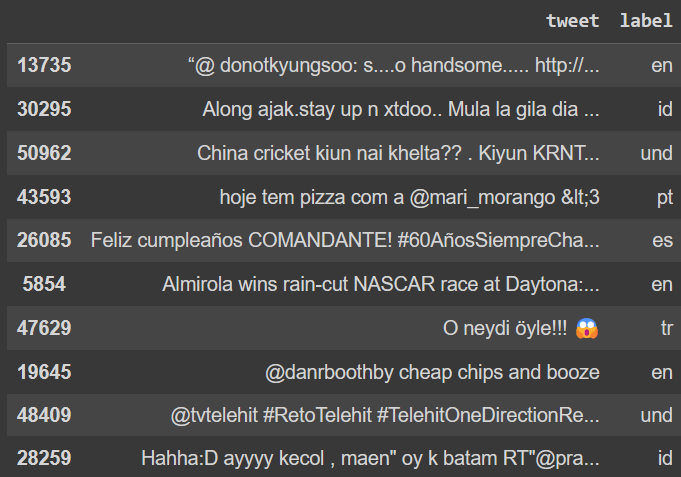
\includegraphics[width=\linewidth]{original_data}
	\caption{Messy Data: Smileys, \# and @ are not language-specific.}
	\label{fig:results}
\end{figure}

\begin{figure}[ht]\centering
	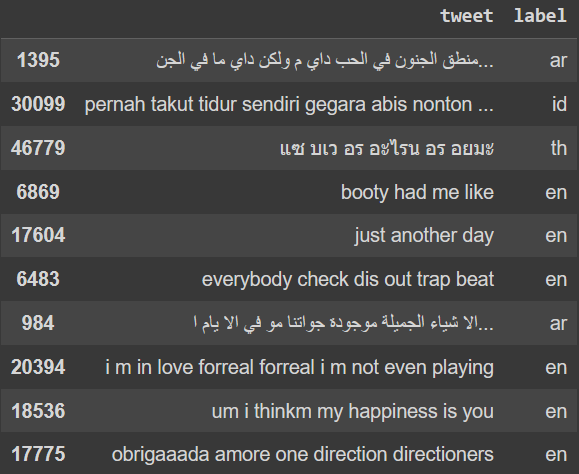
\includegraphics[width=\linewidth]{cleaned_data}
	\caption{Cleaned data: Data which was run through our custom data cleaning pipeline.}
	\label{fig:results}
\end{figure}

\subsection{Data Augmentation}

Looking at the distribution of labels in the data, it is apparent that some labels are severely underrepresented (see Figure 3). For example, the labels "tn," "dv," "ta\_LATN," "si," and "ko\_LATN" are each found in only one of 52675 Twitter posts. To address this issue, it would probably be best to download more data with the underrepresented labels. However, assuming that our data set is a representative sample of all Twitter data, this would unfortunaltely not be computationally feasible. Suppose the training dataset has 52675 observations and some labels are represented only once. To get about 1000 examples of an underrepresented label, one would need to download $52675 * 1000 = 52,675,000$ tweets. Not to mention that one would probably find even rarer labels in the new data, which would then have to be considered as well. \newline

Since it is not possible to download more data for the reasons mentioned above, Data Augmentation (DA) techniques can be used to artificially augment the underrepresented labels. The problem here is that many DA techniques for NLP require language-specific datasets. Exempli gratia, Back-Translation (BT) uses Deep Neural Nets trained on specific languages to translate a document into another language. The translated document is then back-translated into the corresponding original language. Since the languages of underrepresented labels are rarely spoken, it is unlikely to find such translators for all of them. \newline

To address this, we have identified two augmentation techniques that work in a relatively language-independent manner. The two techniques are:
\begin{itemize}
	\item Random Deletion (RD): RD randomly deletes one or more words from a given string.
	\item Random Swap (RS): RS randomly swaps two or more words in a given string.
\end{itemize}

It is evident that these two techniques are rather weak in oppose to BT. This further becomes clear when looking at the confusion matrix in Appendix 1 \& 2. The underrepresented labels of the training data set were, if they were even contained in the test set, not accurately predicted. Further explanation can be found in the results section. \newline

We defined that each label must appear at least a thousand times in the training dataset. To boost the underrepresented labels, we used the following procedure:
\begin{enumerate}[noitemsep]
	\item Identify all languages, where less than 1000 tweets exist in the training data set.
	\item Identify the number N of up-samples that must be performed to obtain 1000 labels (e.g. The training data set contains 981 tweets in Albanian. --> 1000-981 = 19 tweets must be augmented).
	\item Randomly choose N tweets in a given language and augment them.
	\item Append these augmented tweets to the training data set.
\end{enumerate}
This procedure was packed inside a Python Object to simplify the application. The augmented dataset contained 107627 tweets. 


\begin{figure}[ht]\centering
	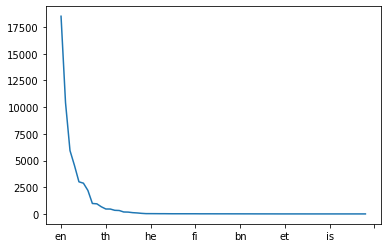
\includegraphics[width=\linewidth]{label_distribution}
	\caption{Label Distribution: Some of the languages are grossly underrepresented in the dataset.}
	\label{fig:results}
\end{figure}

\subsection{Feature Engineering}

"Feature engineering is one of the most important steps in machine learning. It is the process of using domain knowledge of the data to create features that make machine learning algorithms work." (https://www.analyticsvidhya.com/blog/2021/04/\newline a-guide-to-feature-engineering-in-nlp/). We vectorized the cleaned and augmented data set using sklearn CountVectorizer. We also included the Term Frequency-Inverse Document Frequency (TFIDF) metric so that our machine learning models could better detect the variations in meaning between different tweets. For this, we used sklearn TfidfTransformer. To reduce Training Time we also sampled down the number of predictors to 50000 using sklearn SelectKBest with a chi squared test

Furthermore an additional feature was added: We hypothesized that the mean length of tweets of different languages might vary, as some languages have shorter overall mean word length than others. For that purpose we created our own sklearn class and added it to the training pipeline.

\section{Model Training}

In the following, we outline our machine learning setting, followed by remarks on the Baseline Model and the Deep Neural Net Model.

\subsection{Cross-Validation and General Remarks on Model Training}

\paragraph{Train-Test-Split} The augmented training data set was split into a training and a validation data set. For that purpose we used the train\_test\_split function from sklearn. To keep the two data sets balanced, we shuffled the data before the split. We assigned 90\% of the data to the training data set and 10\% of the data to the validation data set. After the split, the training set contained 96864 observations and the validation set 10763 observations. By obvious reasons we did not put our hands on the test data set.

\paragraph{Cross-Validation}
We used Repeated K-Fold Cross Validation (RCV) to get robust estimates of the models accuracy. RCV repeatedly splits the training data into train and validation sets, estimates the model on the training set and evaluates the accuracy on the validation set. The "mean result [of the accuracy] is expected to be a more accurate estimate of the true unknown underlying mean performance of the model on the dataset, as calculated using the standard error." (https://machinelearningmastery.com/repeated-k-fold-cross-validation-with-python/).

\paragraph{Pipeline Training} We used Pipeline from sklearn to train our models. This is helpful as we wanted to tune the hyper-parameters of the CountVectorizer as well. Note however that we did not add our custom preprocessing function to the pipeline (which could be done with FunctionTransformer() from sklearn). We believe that this would lead to overhead, since it has no hyper-parameters to estimate. By tuning the hyper-parameters of the pipeline, this function would be recomputed with every possible combination of the hyper-parameter grid. By leaving it out of the pipeline this function has a runtime of $O(1)$, by including it, it would have a runtime of $O(\prod\limits_{i = 1}^{n} m_{i,\theta})$, with $ m_i \in \mathbb{N} > 0$ being the number of possible specifications of hyper-parameter $\theta_i$.

\paragraph{Hyper-parameter Tuning}For hyper-parameter-tuning we used GridSearchCV from sklearn using three-fold cross validation. We allowed for the following parameters to vary:
\begin{table}[hbt]
	\caption{Table of possible hyper-parameters}
	\centering
	\begin{tabular}{llr}
		\toprule
		 Function & Parameter & Allowed \\
		\midrule
		CountVectorizer & ngram\_range & $(1,1), (1,2)$ \\
		CountVectorizer & analyzer & $"word", "char"$ \\
		LogisticRegression & penalty & $"l1", "none"$ \\
		LogisticRegression & solver & $"liblinear", "saga"$ \\
		NNet & activation & $"idnetity", "logistic"$\\
		NNet & solver & $"lbfgs", "sgd"$ \\
		NNet & early\_stopping & "True"\\
		\bottomrule
	\end{tabular}
	\label{tab:label}
\end{table}


\subsection{Logistic Regression}
Logistic Regression was used to establish a baseline for the Deep Neural Net to beat. The implementation from sklearn automatically one-hot-encodes the criterion, such that we did not have to include this step in our pipeline.

\paragraph{What is logistic regression? - A quick explanation from IBM} "This type of statistical model (also known as logit model) is often used for classification and predictive analytics. Logistic regression estimates the probability of an event occurring, such as voted or didn’t vote, based on a given dataset of independent variables. Since the outcome is a probability, the dependent variable is bounded between 0 and 1. In logistic regression, a logit transformation is applied on the odds—that is, the probability of success divided by the probability of failure. This is also commonly known as the log odds, or the natural logarithm of odds, and this logistic function is represented by the following formulas:

\begin{equation}Logit(\pi) = 1/(1+ exp(-\pi))\end{equation}

\begin{equation}ln(\pi/(1-\pi)) = \beta_0 + \beta_1*X_1 + … + \beta_k*K_k\end{equation}

In this logistic regression equation, $logit(\pi)$ is the dependent or response variable and x is the independent variable. The beta parameter, or coefficient, in this model is commonly estimated via maximum likelihood estimation (MLE). This method tests different values of beta through multiple iterations to optimize for the best fit of log odds. All of these iterations produce the log likelihood function, and logistic regression seeks to maximize this function to find the best parameter estimate. Once the optimal coefficient (or coefficients if there is more than one independent variable) is found, the conditional probabilities for each observation can be calculated, logged, and summed together to yield a predicted probability. For binary classification, a probability less than .5 will predict 0 while a probability greater than 0 will predict 1.  After the model has been computed, it’s best practice to evaluate the how well the model predicts the dependent variable, which is called goodness of fit. The Hosmer–Lemeshow test is a popular method to assess model fit." (https://www.ibm.com/topics/logistic-regression)

\subsection{Deep Neural Net}

\paragraph{What is a Multilayered Perceptron? - A quick explanation from IBM} "Neural networks, also known as artificial neural networks (ANNs) or simulated neural networks (SNNs), are a subset of machine learning and are at the heart of deep learning algorithms. Their name and structure are inspired by the human brain, mimicking the way that biological neurons signal to one another.

Artificial neural networks (ANNs) are comprised of a node layers, containing an input layer, one or more hidden layers, and an output layer. Each node, or artificial neuron, connects to another and has an associated weight and threshold. If the output of any individual node is above the specified threshold value, that node is activated, sending data to the next layer of the network. Otherwise, no data is passed along to the next layer of the network.

Neural networks rely on training data to learn and improve their accuracy over time. However, once these learning algorithms are fine-tuned for accuracy, they are powerful tools in computer science and artificial intelligence, allowing us to classify and cluster data at a high velocity. Tasks in speech recognition or image recognition can take minutes versus hours when compared to the manual identification by human experts. One of the most well-known neural networks is Google’s search algorithm. (https://www.ibm.com/cloud/learn/ \newline neural-networks)

\section{Results and Discussion}
The results section is structured into two parts. First we describe results from the baseline model, second we describe the results from the Deep Neural Net model.

\subsection{Baseline Model}
The following accuracy scored were observed from the baseline model:

\begin{table}[hbt]
	\caption{Accuracy Table}
	\centering
	\begin{tabular}{llr}
		\toprule
		 Data Set & Accuracy & Variance\\
		\midrule
		Training Data Set & 0.929\\
		Validation Data Set & 0.913\\
		Test Data Set & 0.847 \\
		Repeated 2-Fold CV & 0.896 & 0.002\\
		\bottomrule
	\end{tabular}
	\label{tab:label}
\end{table}

The lower accuracy on the test data set in comparison to the training data set in Table 2 is an indication of over-fitting. The more robust estimate of the RCV is closer to the estimate of the test data set. Overall, we conclude that the baseline model has some predictive power. That is, it would outperform a model that allocates all the data to the most represented label of the training dataset (in our case English (en) with 18508 observations). 

The hyper-parameter tuning resulted in the following optimal parameter combination, which was retrieved using sklearn .best\_params\_.

\begin{table}[hbt]
	\caption{Optimal Parameters According to Hyper-Parameter Tuning}
	\centering
	\begin{tabular}{llr}
		\toprule
		 Parameter Name &  Selected Parameter\\
		\midrule
		ngram\_range & (1,1) \\
		analyzer & "word" \\
		penalty & "None" \\
		solver & "liblinear" \\
		\bottomrule
	\end{tabular}
	\label{tab:label}
\end{table}

\paragraph{Why use grid search cross validation?} Hyper-parameter optimization is a difficult task and can quickly lead to over-fitting. That is, the parameter combination found to be optimal during grid search, is fitting very well to the training data, but not to the test data. It is therefore of great importance to get good, robust metric estimates when choosing a hyper-parameter combination. To achieve such robustness, cross validation on the hyper-parameter-tuner can be used. GridSearchCV from sklearn provides users with this functionality (argument: cv = X). 

\paragraph{Performance Evaluation using the Confusion Matrix.} From the confusion matrices in Appendix 1 \& 2, computed on the test data set, it becomes evident that the model performed decent. Most of the classified labels are on the main diagonal, which indicates accurate prediction. There are also some labels that were predicted far to often. These can be identified as the vertical colored "lines" in Appendix 1 (e.g. labels "de" and "hi\_latn"). The proximate explanation is that the model simply assigns tweets to these two labels when it cannot accurately assign them otherwise.

\paragraph{Performance Evaluation using the Classification Report.} As can be interpreted from the classification report, the model performed exceptionally well on languages that come with its own set of "letters" (signs). Exampli gratia, the label "ar" (Arabian) was predicted with 0.99\% accuracy and the label "ru" (Russian), which was by the way subject to augmentation, was predicted with 0.99\% accuracy. Furthermore, labels that are strongly represented in the training data set show good accuracy. For Example, English (en) was predicted with 0.95\% accuracy and Spanish (es) was predicted with 0.90\% accuracy. A closer look at the labels that were severely underrepresented, e.g., with only one observation in the training data, reveals that data augmentation worked very poorly in these cases. For example, in ko\_LATN or ta\_LATN, the one observation that was present in the test data was incorrectly predicted.

\begin{figure}[ht]\centering
	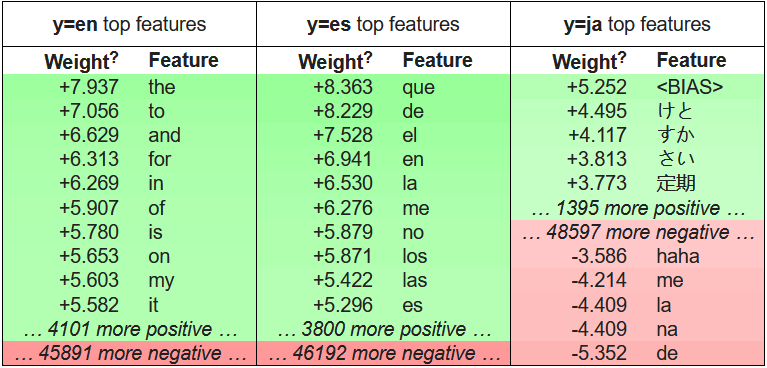
\includegraphics[width=\linewidth]{feature_importance}
	\caption{Feature Importance: Displayed are the top ten most important features and their coefficients.}
	\label{fig:results}
\end{figure}

\paragraph{Most Important Features} Figure 4 shows the ten most important features for the languages English (en), Spanish (es) and Japanese (ja). This table was extracted with the \linebreak show\_weights() function from the ELI5 library. For all of these languages our custom feature (i.e. the length of tweet metric) wasn't among the top ten. We therefore conclude that the mean word length of a tweet is not as important for the classification of these three languages as the bag of words itself.

\subsection{Deep Neural Net Model}
The following accuracy was observed when using the Deep Neural Net model (or non-linear MLP):
\begin{table}[hbt]
	\caption{Accuracy Table}
	\centering
	\begin{tabular}{llr}
		\toprule
		 Data Set & Accuracy & Variance\\
		\midrule
		Training Data Set & 0.331 \\
		Validation Data Set & 0.328\\
		Test Data Set & 0.656 \\
		Repeated 2-Fold CV & 0.310 & 0.004\\
		\bottomrule
	\end{tabular}
	\label{tab:label}
\end{table}\newline
The major difference in accuracy on the test data set in comparison to the training data set in Table 4 can probably be attributed to coincidence. The hyper-parameter tuning of the Deep Neural Net model resulted in the following optimal parameter combination, which was retrieved using sklearn.best.params (note that the accuracy is really low, therefore the parameters are not expected to be robust):\newline
\begin{table}[hbt]
	\caption{Optimal Parameters According to Hyper-Parameter Tuning}
	\centering
	\begin{tabular}{llr}
		\toprule
		 Parameter Name &  Selected Parameter\\
		\midrule
		ngram\_range & (1,1) \\
		analyzer & "word" \\
		activation & "identity" \\
		solver & "lbfgs" \\
        early\_stopping & True \\
		\bottomrule
	\end{tabular}
	\label{tab:label}
\end{table}\newline

\section{Conclusion}
Using the same data splits as in Part 1 of this exercise resulted in a significantly longer run time and less accurate results when compared to the linear classification model. This comparison is, of course, not very fair, as we had to drastically cut model-parameters to optimize for computational workload. We believe that model depth (around 150 deep layers) would play a key role when trying to achieve better accuracy. According to our results, we would choose the Logistic Regression Model as it had better performance. However, if we had more computing power, we believe that the Neural Net could have outperformed the Logistic Regression Model. We leave that up to further research.
\section{Appendix}

\begin{figure*}[ht]\centering % Using \begin{figure*} makes the figure take up the entire width of the page
	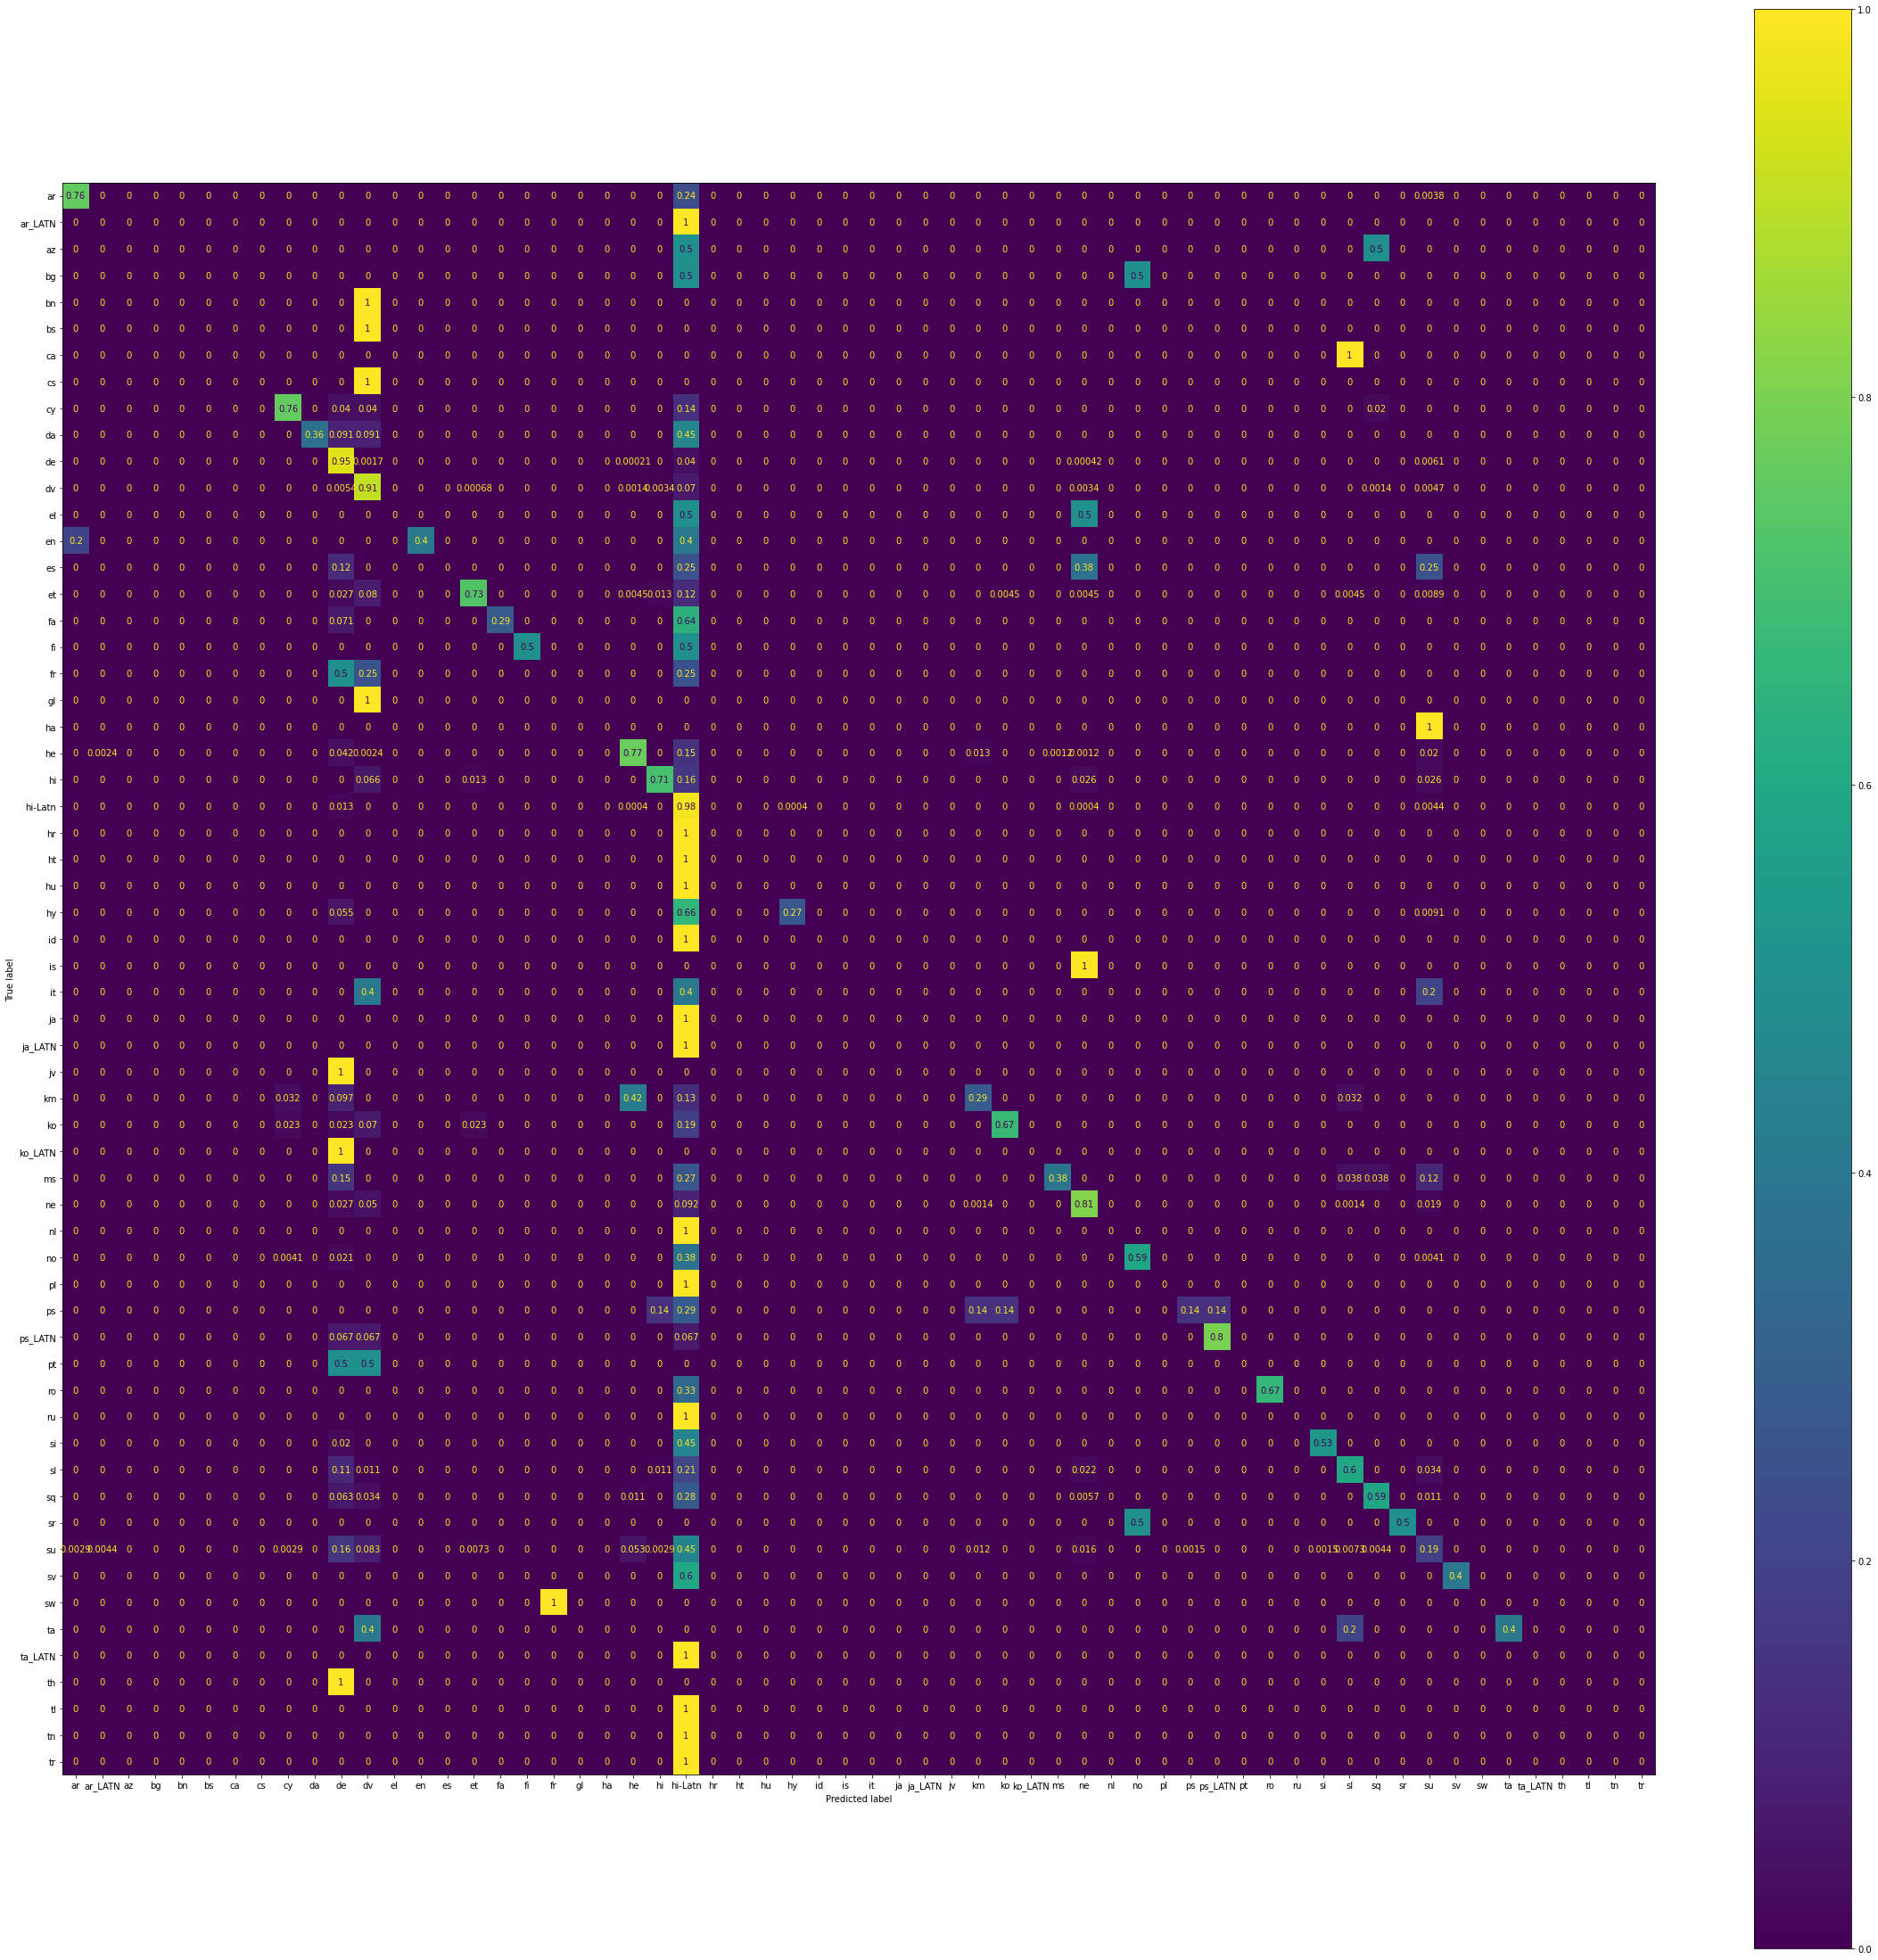
\includegraphics[width=\linewidth]{confusion_matrix_normalized}
	\caption{Confusion Matrix of the Test Data Set (Normalized)}
	\label{fig:view}
\end{figure*}

\begin{figure*}[ht]\centering % Using \begin{figure*} makes the figure take up the entire width of the page
	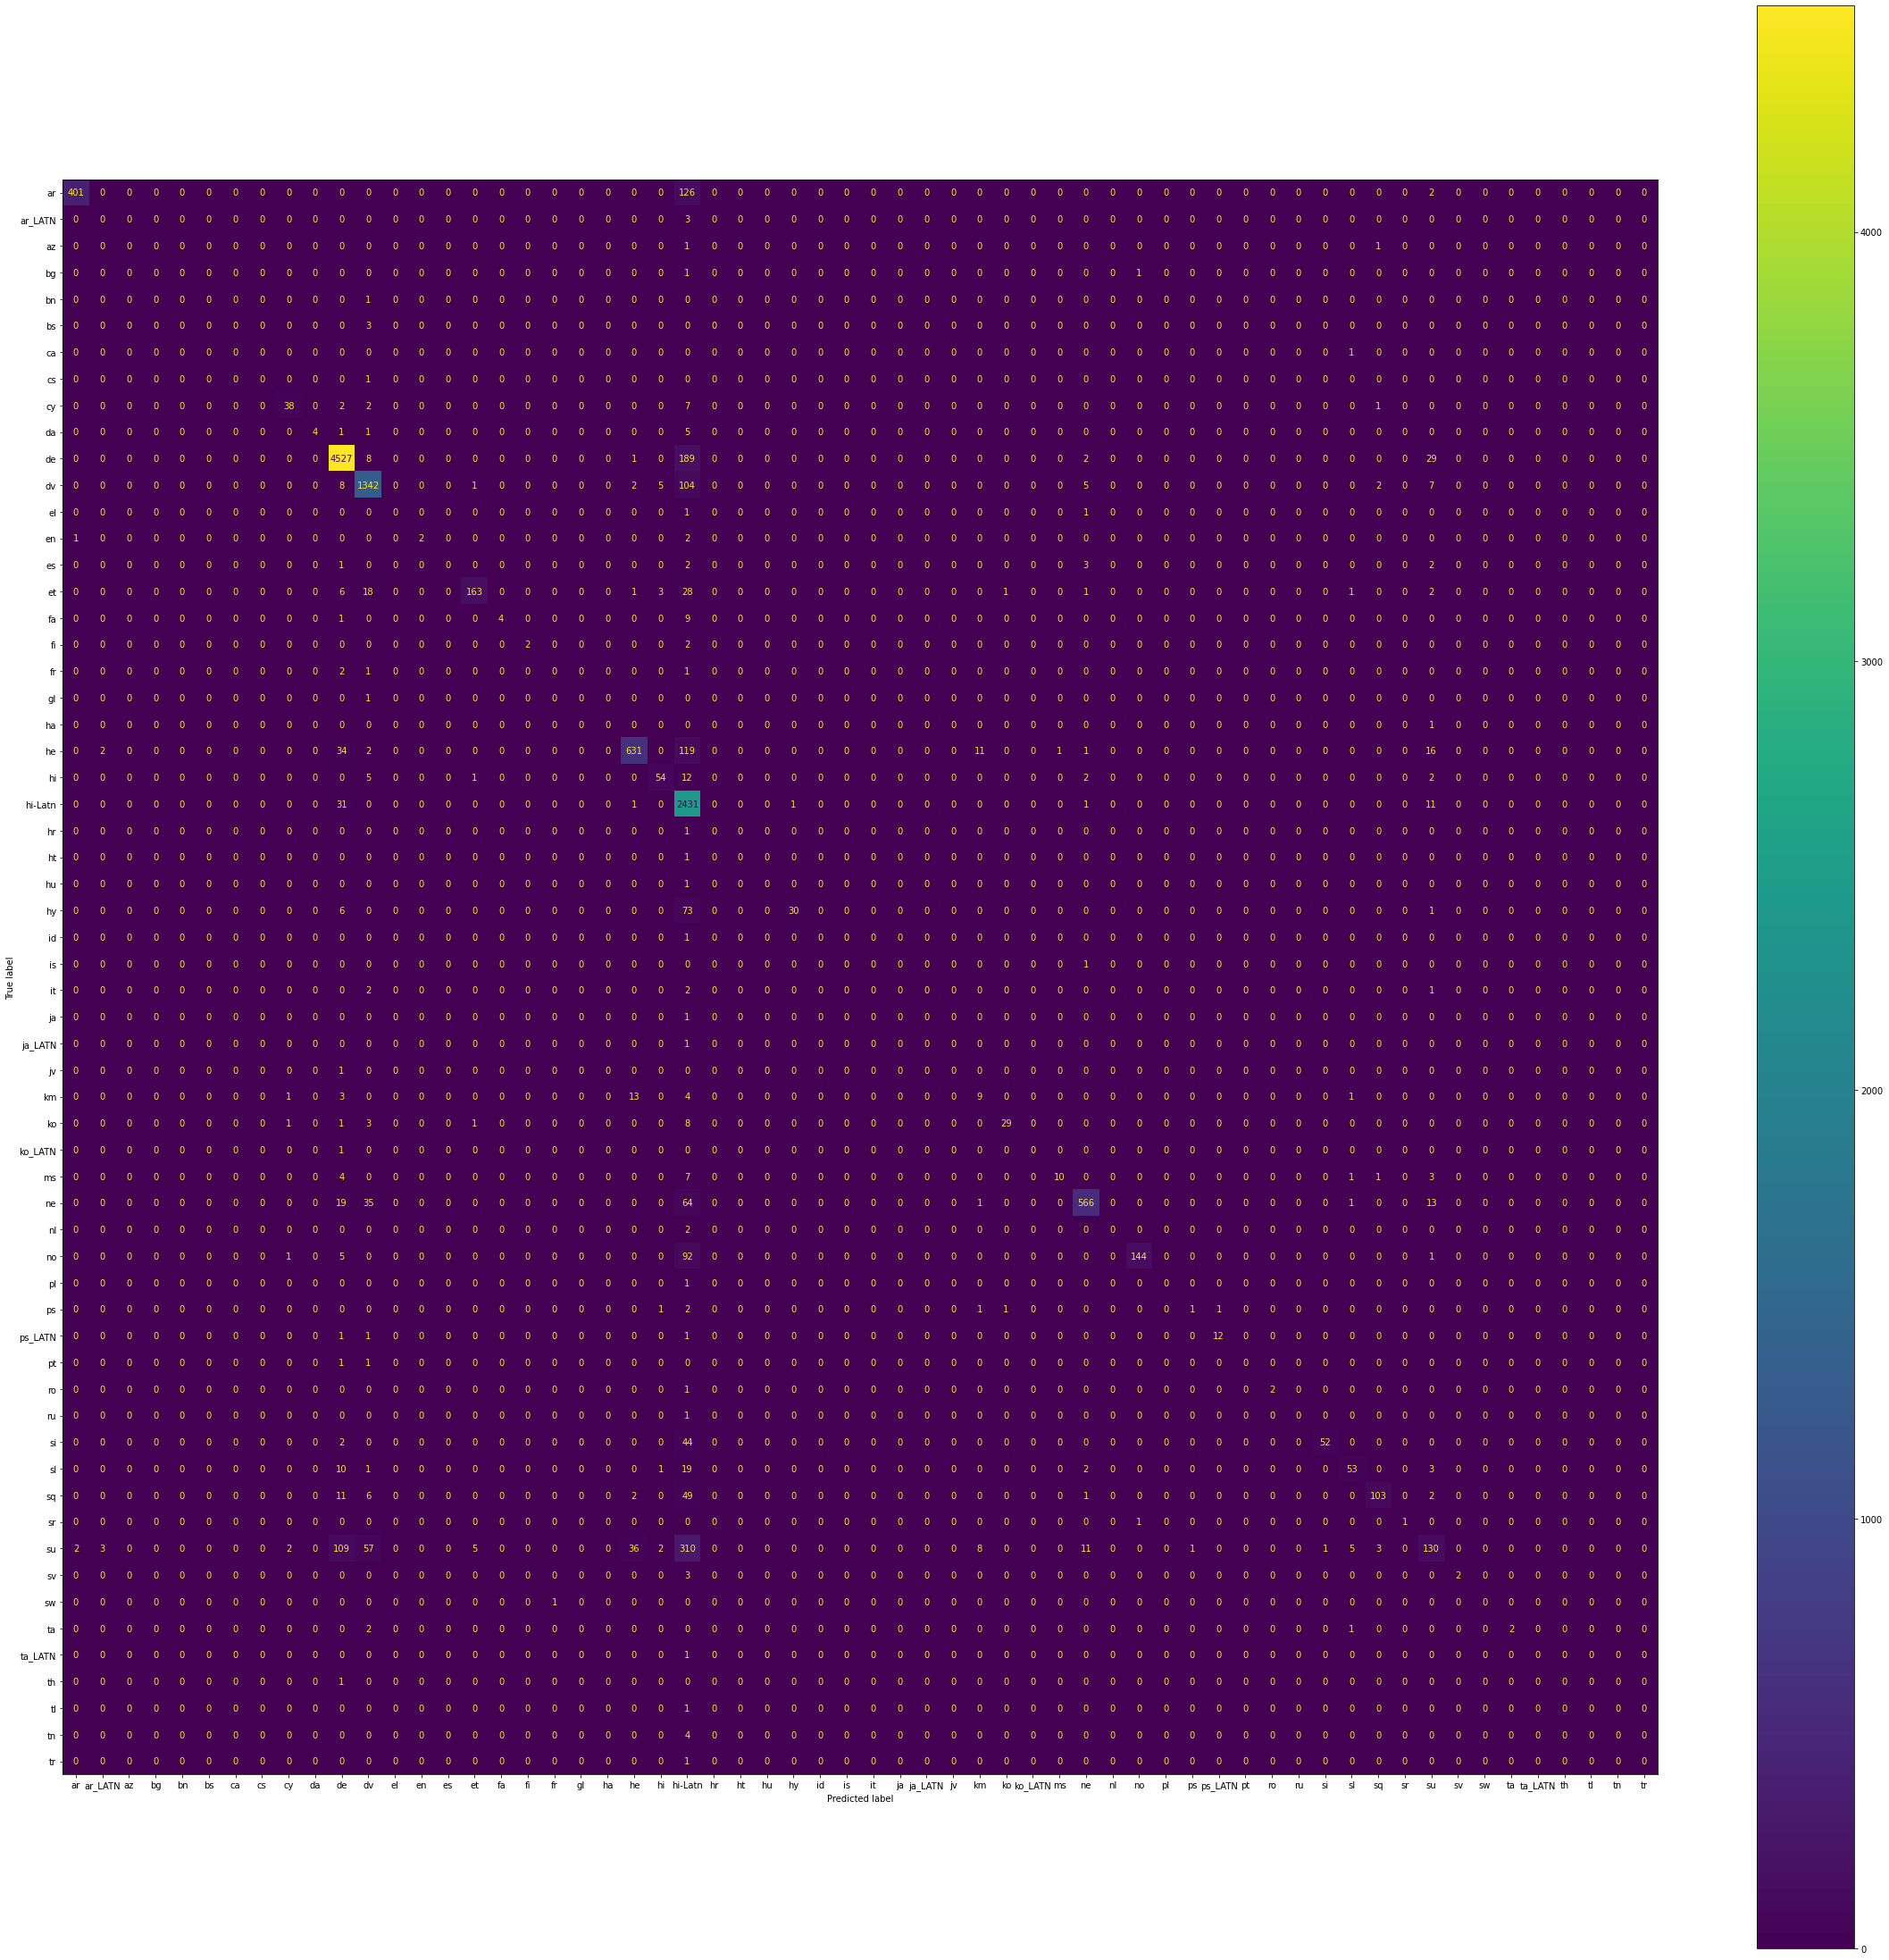
\includegraphics[width=\linewidth]{confusion_matrix_not_normalized}
	\caption{Confusion Matrix of the Test Data Set (Not Normalized)}
	\label{fig:view}
\end{figure*}

\begin{table*}[hbt]
	\caption{Classification Report for the Testing Data Set 1/2}
	\centering
	\begin{tabular}{llllr}
	\toprule
	Language & Precision & Recall  & F1-score & Support \\
	\midrule
	ar & 0.99 & 0.76 & 0.86 & 529\\
	ar\_LATN & 0.00 & 0.00 & 0.00 & 3\\
	az & 0.00 & 0.00 & 0.00 & 2\\
	bg & 0.00 & 0.00 & 0.00 & 2\\
	bs & 0.00 & 0.00 & 0.00 & 1\\
	ca & 0.00 & 0.00 & 0.00 & 3\\
	cs & 0.00 & 0.00 & 0.00 & 1\\
	da & 0.00 & 0.00 & 0.00 & 1\\
	de & 0.86 & 0.76 & 0.81 & 50\\
	el  & 1.00 & 0.36 & 0.53 & 11\\
	en & 0.95 & 0.95 & 0.95 & 4756\\
	es & 0.90 & 0.91 & 0.90 & 1476\\
	eu & 0.00 & 0.00 & 0.00 & 2\\
	fa & 1.00 & 0.40 & 0.57 & 5\\
	fi & 0.00 & 0.00 & 0.00 & 8\\
	fr & 0.96 & 0.72 & 0.82 & 224\\
	he & 1.00 & 0.29 & 0.44 & 14\\
	hi & 1.00 & 0.75 & 0.86 & 4\\
	hi-Latn & 0.00 & 0.00 & 0.00 & 4\\
	hr & 0.00 & 0.00 & 0.00 & 1\\
	ht & 0.00 & 0.00 & 0.00 & 1\\
	id & 0.92 & 0.77 & 0.84 & 817\\
	it & 0.85 & 0.72 & 0.78 & 76\\
	ja & 0.64 & 0.98 & 0.78 & 2476\\
	ja\_LATN & 0.00 & 0.00 & 0.00 & 1\\
	jv & 0.00 & 0.00 & 0.00 & 1\\
	km & 0.00 & 0.00 & 0.00 & 1\\
	ko  & 0.96 & 0.23 & 0.37 & 110\\
	ko\_LATN & 0.00 & 0.00 & 0.00 & 1\\
	la & 0.00 & 0.00 & 0.00 & 1\\
	lv & 0.00 & 0.00 & 0.00 & 5\\
	mk & 0.00 & 0.00 & 0.00 & 1\\
	mn & 0.00 & 0.00 & 0.00 & 1\\
	mr & 0.00 & 0.00 & 0.00 & 1\\
	ms & 0.30 & 0.29 & 0.30 & 31\\
	nl & 0.93 & 0.65 & 0.77 & 43\\
	no & 0.00 & 0.00 & 0.00 & 1\\
	pl & 0.85 & 0.42 & 0.56 & 26\\
	pt & 0.95 & 0.81 & 0.87 & 699\\
	ro & 0.00 & 0.00 & 0.00 & 2\\
	ru & 0.99 & 0.59 & 0.74 & 243\\
	sk & 0.00 & 0.00 & 0.00 & 1\\
	sr & 0.00 & 0.00 & 0.00 & 7\\
	sv & 0.92 & 0.80 & 0.86 & 15\\
	sw & 0.00 & 0.00 & 0.00 & 2\\
	ta  & 1.00 & 0.67 & 0.80 & 3\\
	ta\_LATN & 0.00 & 0.00 & 0.00 & 1\\
      \bottomrule
	\end{tabular}
	\label{tab:label}
\end{table*}

\begin{table*}[hbt]
	\caption{Classification Report for the Testing Data Set  2/2}
	\centering
	\begin{tabular}{llllr}
	\toprule
	Language & Precision & Recall  & F1-score & Support \\
	\midrule
	th & 0.98 & 0.52 & 0.68 & 98\\
	tl & 0.74 & 0.60 & 0.66 & 89\\
	tr & 0.93 & 0.57 & 0.71 & 174\\
	uk & 1.00 & 0.50 & 0.67 & 2\\
	und & 0.58 & 0.18 & 0.27 & 685\\
	ur & 1.00 & 0.40 & 0.57 & 5\\
	ur\_LATN & 0.00 & 0.00 & 0.00 & 1\\
	vi & 1.00 & 0.60 & 0.75 & 5\\
	xh & 0.00 & 0.00 & 0.00 & 1\\
	yo & 0.00 & 0.00 & 0.00 & 1\\
	zh-CN & 0.00 & 0.00 & 0.00 & 1\\
	zh-TW & 0.00 & 0.00 & 0.00 & 4\\
	zu & 0.00 & 0.00 & 0.00 & 1\\
	\bf accuracy & \bf - & \bf - & \bf 0.84 & \bf 12731 \\
	\bf macro\_avg & \bf 0.40 & \bf 0.27 & \bf 0.31 & \bf 12731 \\
	\bf weighted\_avg & \bf 0.85 & \bf 0.84 & \bf 0.83 & \bf 12731\\
      \bottomrule
	\end{tabular}
	\label{tab:label}
\end{table*}

%----------------------------------------------------------------------------------------

\end{document}